\documentclass{article}%
\usepackage[T1]{fontenc}%
\usepackage[utf8]{inputenc}%
\usepackage{lmodern}%
\usepackage{textcomp}%
\usepackage{lastpage}%
\usepackage[head=40pt,margin=0.5in,bottom=0.6in]{geometry}%
\usepackage{graphicx}%
%
\title{\textbf{Estudiantes de Bioanálisis rechazan  presunto cierre técnico de sus escuelas}}%
\author{MARÍA FERNANDEZ}%
\date{03/12/2018}%
%
\begin{document}%
\normalsize%
\maketitle%
\textbf{URL: }%
http://www.eluniversal.com/caracas/27311/estudiantes{-}de{-}bioanalisis{-}se{-}pronuncian{-}por{-}presunto{-}cierre{-}tecnico{-}de{-}sus{-}escuelas{-}a{-}nivel\newline%
%
\textbf{Periodico: }%
EU, %
ID: %
27311, %
Seccion: %
caracas\newline%
%
\textbf{Palabras Claves: }%
NO\_TIENE\newline%
%
\textbf{Derecho: }%
2.2, %
Otros Derechos: %
, %
Sub Derechos: %
2.2.1\newline%
%
\textbf{EP: }%
NO\newline%
\newline%
%
\textbf{\textit{A través de un comunicado de la Federación Venezolana de Estudiantes de Bioanálisis consideran que esta situación es un gigantesco retraso para la formación de futuros profesionales}}%
\newline%
\newline%
%
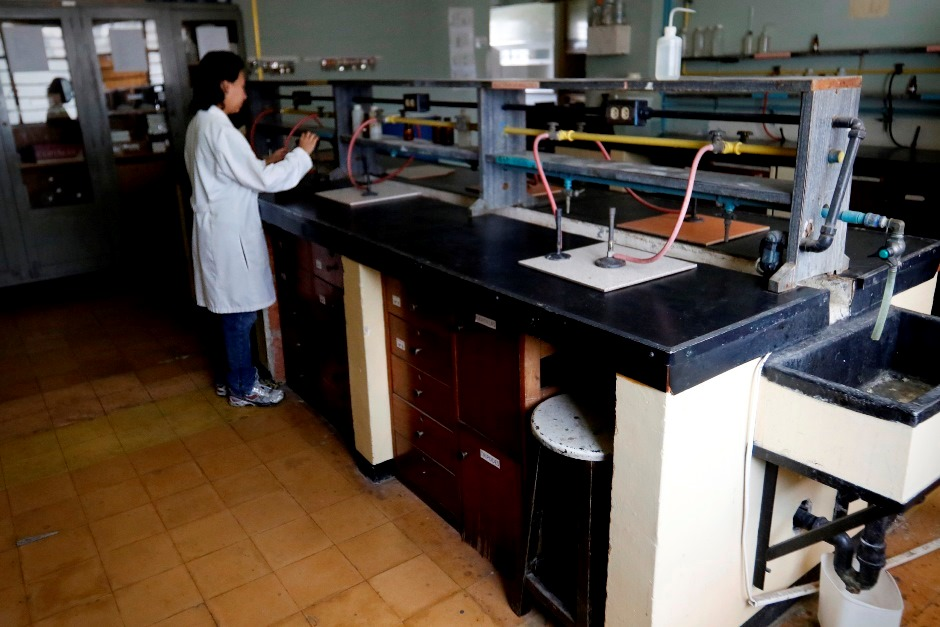
\includegraphics[width=300px]{85.jpg}%
\newline%
%
Estudiantes de Bioanálisis de diferentes Universidades en Venezuela, se pronunciaron sobre un posible cierre técnico~de sus escuelas, por la grave falta de insumos e inseguridad que están~viviendo.%
\newline%
%
Comunicado Federación Venezolana de Estudiantes de Bioanálisis.%
\newline%
%
La Federación Venezolana de Estudiantes de Bioanálisis, como representación de distintas universidades a nivel nacional, expresamos la situación tan precaria que vivimos como estudiantes, donde solamente el Gobierno Nacional es culpable del ocaso de nuestra educación. En todo el territorio venezolano presentamos las siguientes problemáticas que impulsan a un lamentable cierre técnico:%
\newline%
%
1.{-} La crisis del sector salud, nos afecta de manera directa, donde la falta de reactivos e insumos médicos en los laboratorios hace difícil cumplir nuestra función con la sociedad civil, sumando la falta de equipos tecnológicos y su respectivo mantenimiento impiden la realización de las prácticas que realizamos a diario.%
\newline%
%
2.{-} El alto grado de inseguridad dentro de nuestras Casas de Estudio, en donde diariamente somos víctimas de las bandas delictivas, que no creen en la Academia como base fundamental de la sociedad.%
\newline%
%
3.{-} La alta deserción estudiantil y profesoral, ocasiona un gigantesco retraso para la formación de futuros profesionales en el área del Bioanálisis en el territorio nacional.%
\newline%
%
4.{-} Las becas Estudiantiles son una miseria, las cuales no se ajustan a la realidad que viven a diario los estudiantes de nuestras Escuelas.%
\newline%
%
5.{-} La grave problemática con el transporte público y la paralización indefinida de las unidades de transportes institucionales, lo que dificulta el traslado de todos los que hacen vida en nuestras comunidades.%
\newline%
%
6.{-} El funcionamiento casi inexistente del servicio de Comedor Universitario, recordando que es una ayuda indispensable para el estudiantado y aún más en la situación actual del país.%
\newline%
%
Nosotros como Representantes Estudiantiles electos democráticamente como voceros de nuestra comunidad y protectores de nuestra Alma Mater se nos hace cuesta arriba mantener las puertas abiertas de nuestras Escuelas, en conjunto con nuestras respectivas Autoridades.%
\newline%
%
Queremos pedir el apoyo de los egresados de las diferentes casas de estudio a nivel nacional y sobre todo de los venezolanos, para lograr resurgir en este momento de quiebre máximo, recordando que las Universidades son el músculo de la sociedad civil.%
\newline%
%
\end{document}